% !TEX root = ../zenkoku.tex
\section{結果}
アンケートは部の開発者全員である9人全員から回答を得た.

集計方法としては熟練した開発者を1人想定し,この開発者への依存度が高いようなシステムを洗い出すことにした.
理解度は値が高いほど理解が深いものとし,`熟練者の理解度 - 熟練者を除いた開発者の理解度平均` によって求めた数値を熟練者への属人性の高さとする.

結果を\ri{img:rikai}に示す.


属人性の高さとして 3pt を閾値としたときに

属人性が高いものがn個
低いものhoge個

% TODO: グラフをモノクロで印刷したときに折れ線とか全然わからないので修正したい.
% グラフの種類を階段面にしたら多少マシになるような気もするけどそれはそれで見づらいかも
\begin{figure}
	\centering
	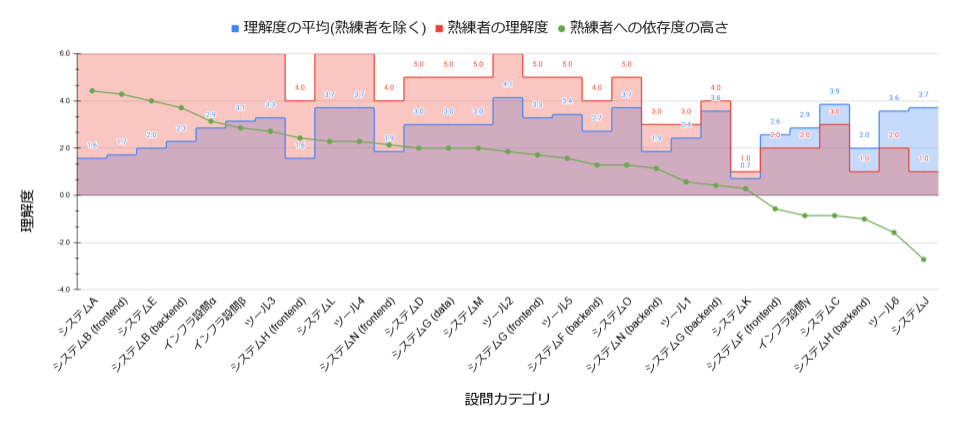
\includegraphics[keepaspectratio,width=0.9\linewidth]{img/rikai.png}
	\caption{システムに対する理解度の平均と依存度の高さ}
	\label{img:rikai}
\end{figure}
